Following the work of \cite{Brosse18tULA}, we aim to quantify the accuracy of these methods by finding the first and second moments of known distributions. Then, comparing the error between the generated value and the true value will give a first indication on the accuracy of the scheme. Beginning with the original code associated with \cite{Brosse18tULA}\footnote{Available at \url{https://github.com/nbrosse/TULA}}, we initially optimised the code then aimed to reproduce the results they found. 

\subsection{Testing Potentials}
For the purposes of testing, four qualitatively different potentials have been made available within our program. These are: Gaussian, Double Well, Rosenbrock function and Ginzburg-Landau model. We note that these, save for Gaussian, are non-convex.

Any of the above potentials may also be scaled by \textit{temperature} $T$. That is, having chosen a potential function $U$ and a temperature $T$, the true distribution to be sampled from will be
\[\pi(x) = e^{-\frac{U(x)}{T}}.\]
This is common in the molecular dynamics literature and is also useful in MCMC to find modes of distributions more quickly, a technique known as tempering.

+++ BoxPlots +++
\begin{figure}
\centering
  \begin{minipage}[b]{0.32\textwidth}
  \centering
    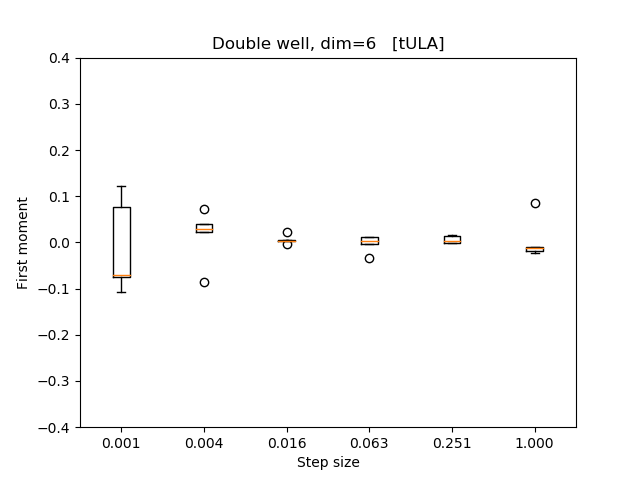
\includegraphics[width=\textwidth]{Figures/tula_fm.png}
  \end{minipage} %
  \begin{minipage}[b]{0.32\textwidth}
  \centering
    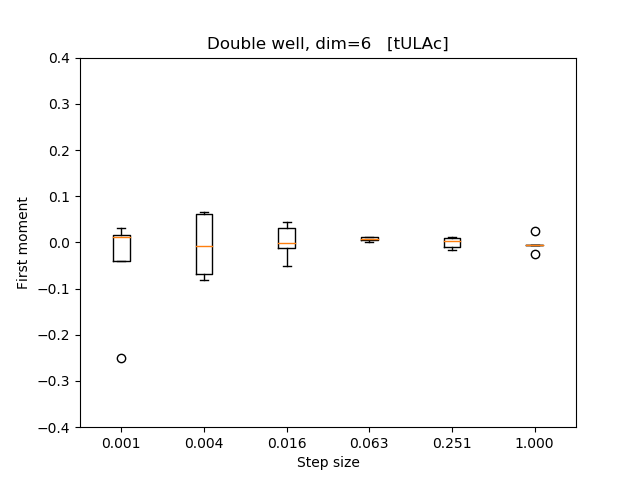
\includegraphics[width=\textwidth]{Figures/tulac_fm.png}
  \end{minipage} %
  \begin{minipage}[b]{0.32\textwidth}
  \centering
    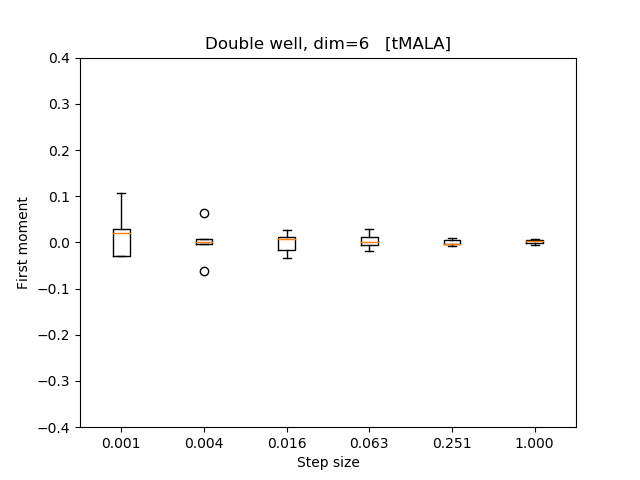
\includegraphics[width=\textwidth]{Figures/tmala_fm.png}
  \end{minipage}
   \caption{Comparison of \texttt{tULA}, \texttt{tULAc} and \texttt{tMALA} for the first moment evolving as a function of step size.}
\end{figure}

\begin{figure}
\centering
  \begin{minipage}[b]{0.85\textwidth}
  \centering
    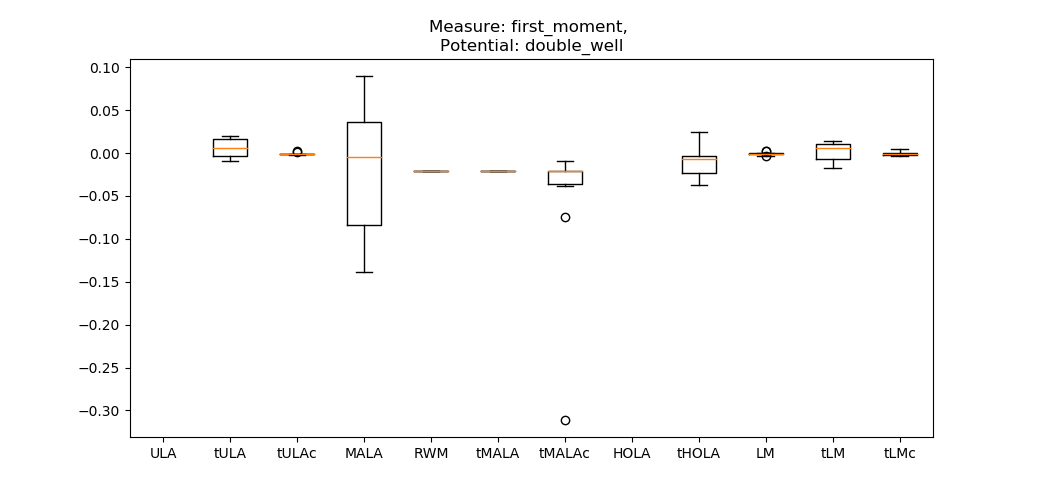
\includegraphics[width=\textwidth]{Figures/doublewell_0_1_10_5samp_100dFirstMoment.png}
  \end{minipage}\\ %
  \begin{minipage}[b]{0.85\textwidth}
  \centering
    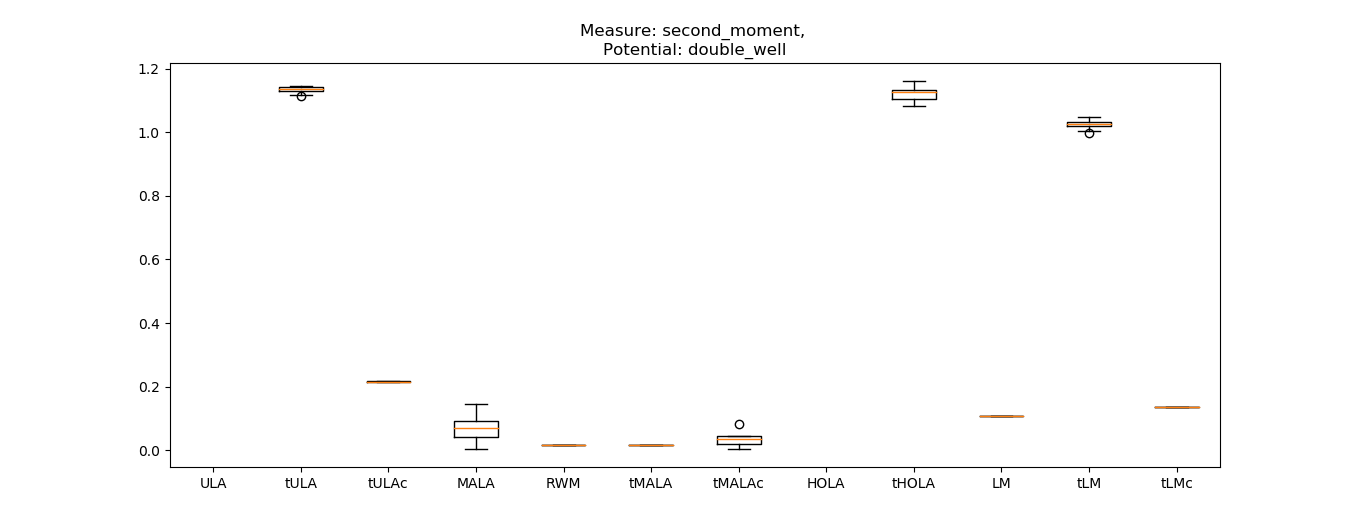
\includegraphics[width=\textwidth]{Figures/secondmoment_double_well_100d_10_5samp.png}
  \end{minipage} %
  \caption{}
  \label{fig:doubleWell_moment}
  \end{figure}